\section{Felix Lase}
\subsection{sejarah}
Python diciptakan oleh Guido van Rossum untuk pertama kalinya di Scitchting Mathematisch Centrum (CWI) di Belanda pada awal 1990-an. Bahasa Python terinspirasi oleh bahasa pemrograman ABC. Sampai sekarang, Guido masih menjadi penulis utama untuk Python, meskipun open source terbuka untuk ribuan orang yang juga berkontribusi pada pengembangannya.
\par
Pada tahun 1995, Guido terus membuat python di Corporate for National Research Initiative (CNRI) di Virginia America, tempat ia merilis beberapa versi Python.
\par
Pada bulan Mei 2000, Guido dan tim Python pindah ke BeOpen.com dan membentuk tim BeOpen PythonLabs. Pada bulan Oktober tahun yang sama, tim Python pindah ke Digital Creation (sekarang Zope Company). Pada tahun 2001, Organisasi Python dibentuk, Yayasan Perangkat Lunak Python (PSF). PSF adalah organisasi nirlaba yang khusus dibuat untuk semua hal yang berkaitan dengan kekayaan intelektual Python. Perusahaan Zope adalah anggota sponsor PSF.
\par
Semua versi Python yang dirilis adalah open source. Dalam sejarahnya, hampir semua rilis python menggunakan lisensi yang kompatibel dengan GFL. Berikutnya adalah versi minor dari walikota dan python bersama dengan tanggal rilis.Instalasi anaconda
\subsection{Instalasi Anaconda}
\begin{enumerate}
    \item Terlebih dahulu kita harus mendownload python, sebelum anaconda diinstal
    \item Buka installer klik Next
     \begin{figure}[!htbp]
        \centering
        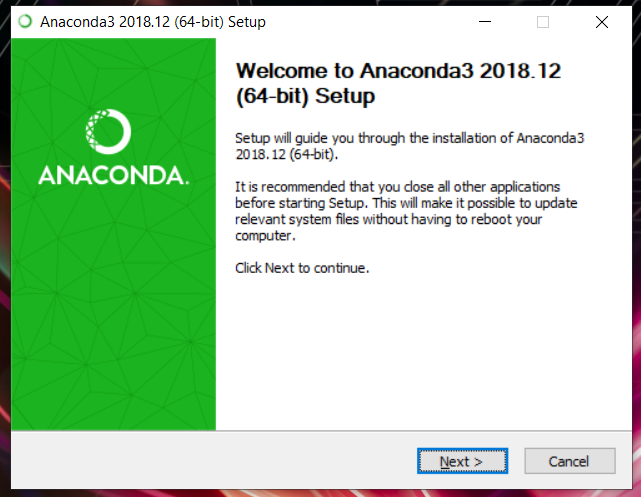
\includegraphics[width=3cm,height=3cm]{figures/1..png}
        \caption{Tampilan Awal}
        \label{awal}
        \end{figure}
    \item Klik I Agree untuk membuka lisensi
     \begin{figure}[!htbp]
        \centering
        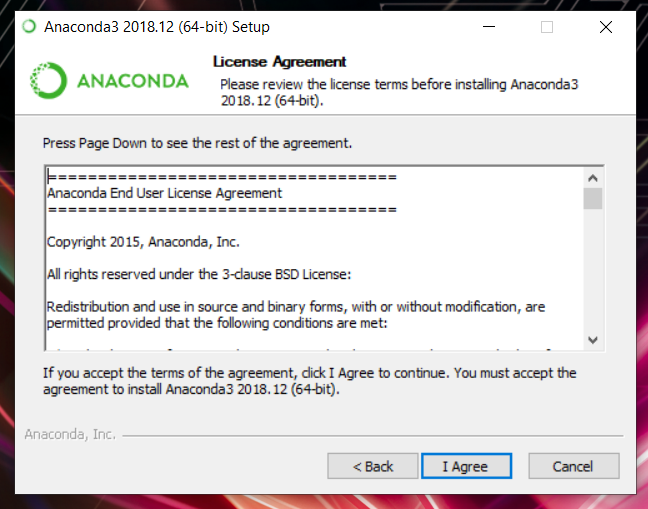
\includegraphics[width=3cm,height=3cm]{figures/2..png}
        \caption{License}
        \label{awal}
        \end{figure}
    \item  Pilih untuk siapa aplikasi diinstal bisa just me dan juga bisa all users
     \begin{figure}[!htbp]
        \centering
        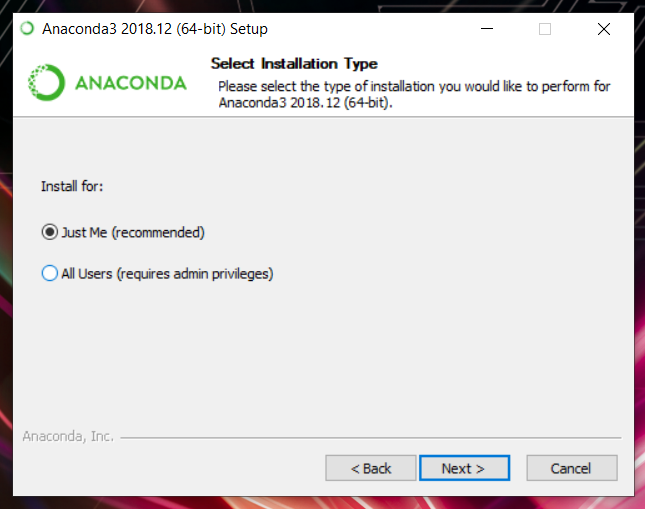
\includegraphics[width=3cm,height=3cm]{figures/3..png}
        \caption{Proses}
        \label{awal}
        \end{figure}
    \item  Pilih lokasi instalasi
    \begin{figure}[!htbp]
        \centering
        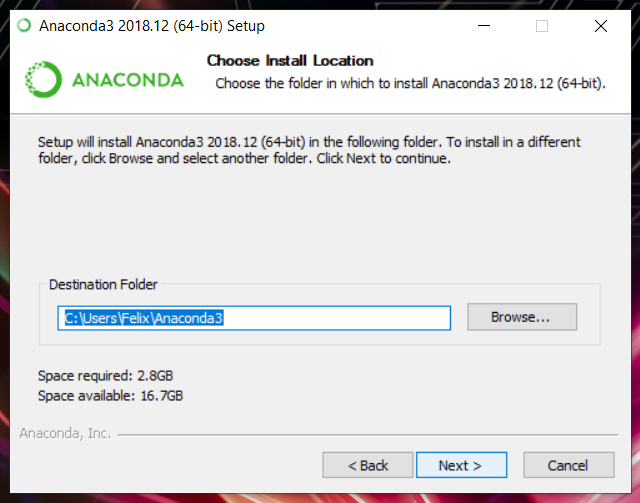
\includegraphics[width=3cm,height=3cm]{figures/4..png}
        \caption{Proses}
        \label{awal}
        \end{figure}
    \item Pilih register anaconda karna add aconda environment tidak remomended
    \begin{figure}[!htbp]
        \centering
        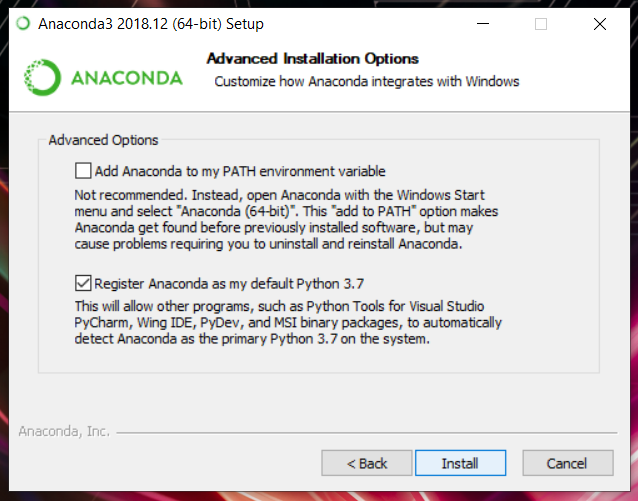
\includegraphics[width=3cm,height=3cm]{figures/5..png}
        \caption{Proses}
        \label{awal}
        \end{figure}
    \item Tunggu hingga selesai
    \begin{figure}[!htbp]
        \centering
        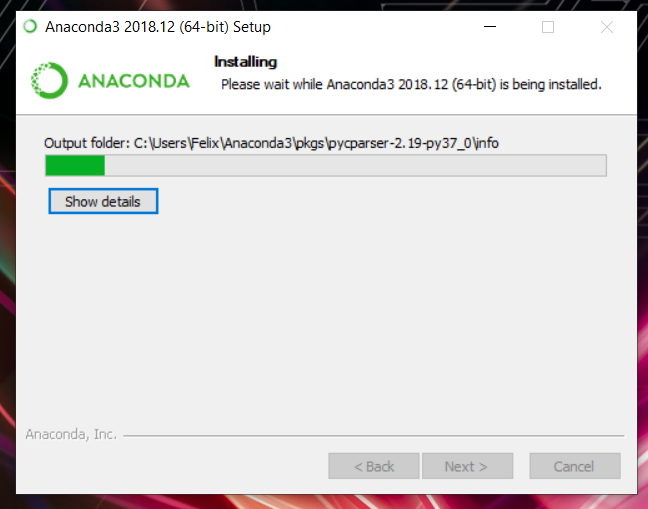
\includegraphics[width=3cm,height=3cm]{figures/6..png}
        \caption{Proses}
        \label{awal}
        \end{figure}
    \item Klik skip
    \begin{figure}[!htbp]
        \centering
        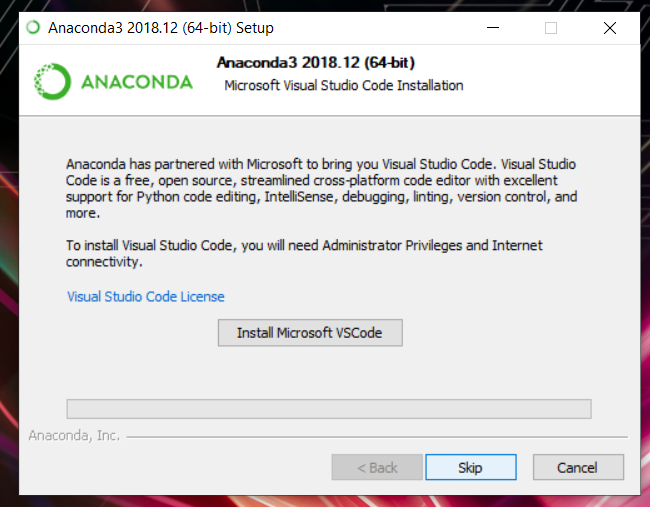
\includegraphics[width=3cm,height=3cm]{figures/8..png}
        \caption{Proses}
        \label{awal}
        \end{figure}
    \item  Dan anaconda berhasil di install
    \begin{figure}[!htbp]
        \centering
        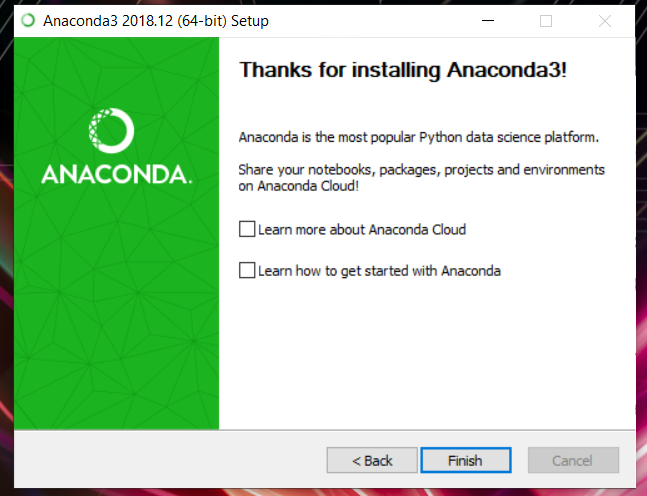
\includegraphics[width=3cm,height=3cm]{figures/9..png}
        \caption{Proses}
        \label{awal}
        \end{figure}
\end{enumerate}
\subsection{Menggunakan Spyder}
setelah selesai menggunakan instalasi anaconda,  maka ada beberapa tool yang digunakan seperti spyder
\begin{figure}[!htbp]
        \centering
        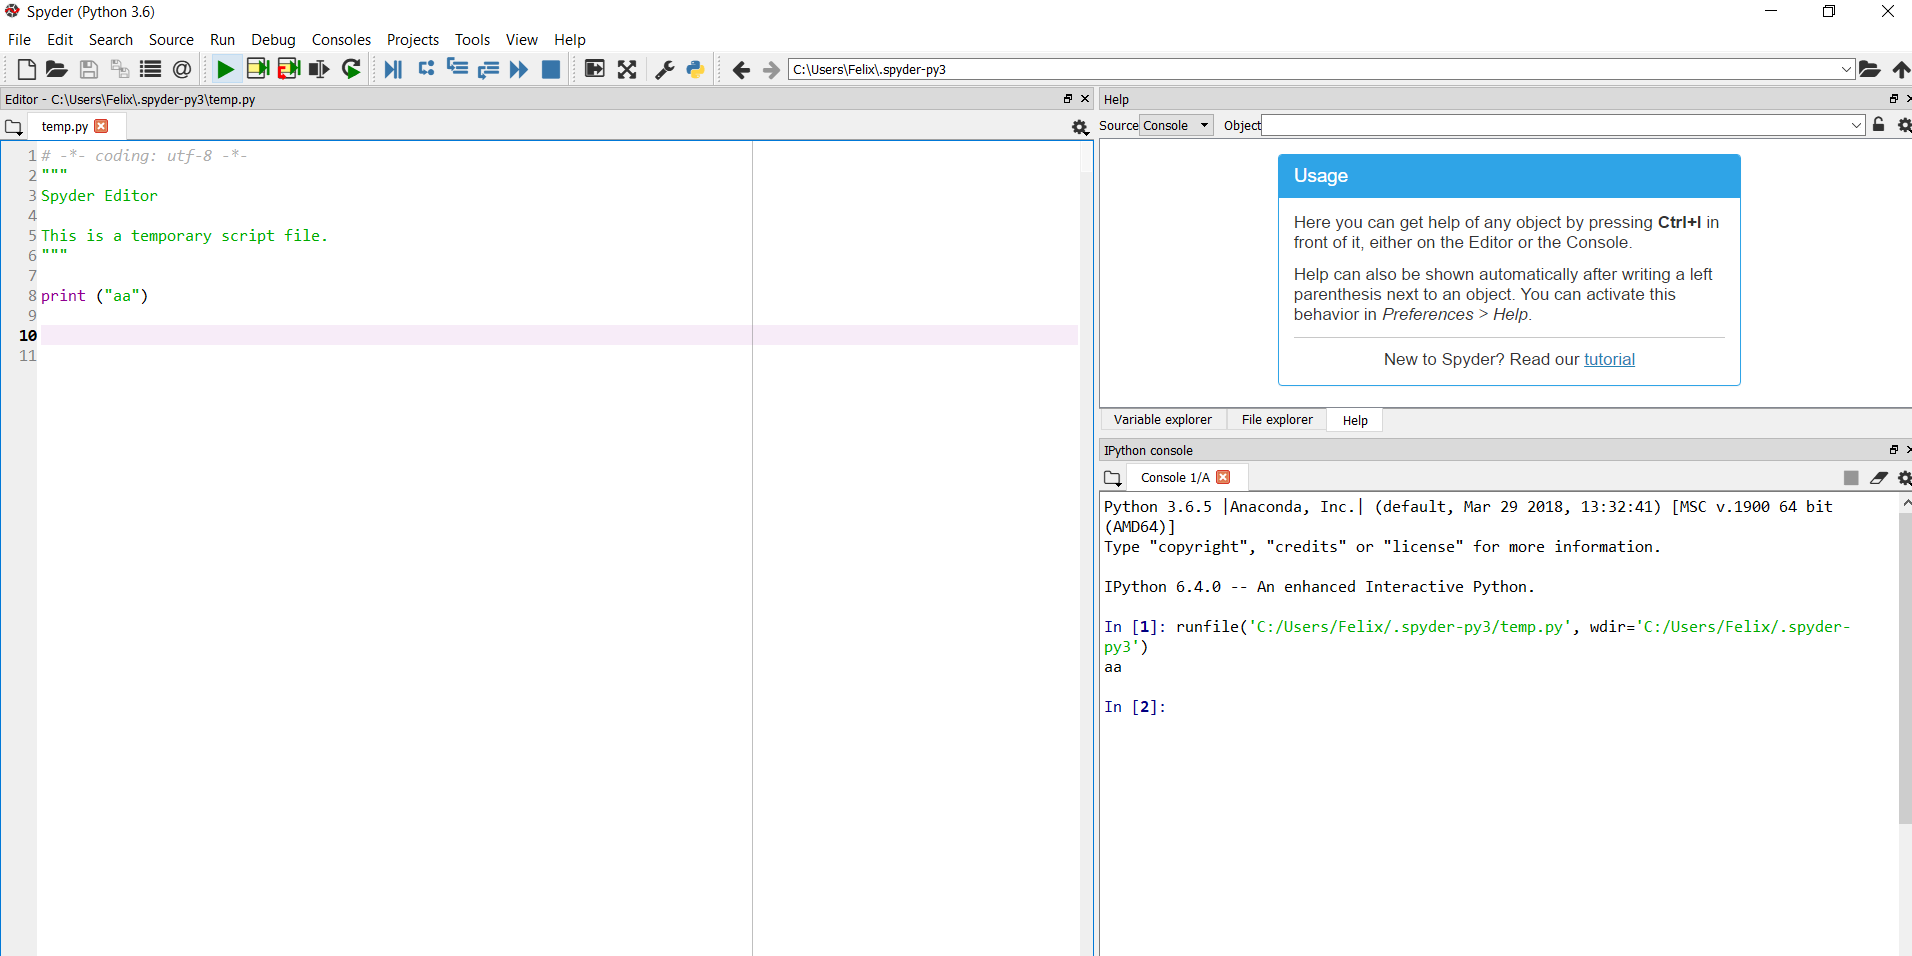
\includegraphics[width=3cm,height=3cm]{figures/10.png}
        \caption{Proses}
        \label{awal}
        \end{figure}

Gambar tersebut menjelaskan tentang tampilan spyder dan mengeksekusi program aa